\begin{tikzpicture}
	\draw(0,0) node [anchor=south west,inner sep=0] (image){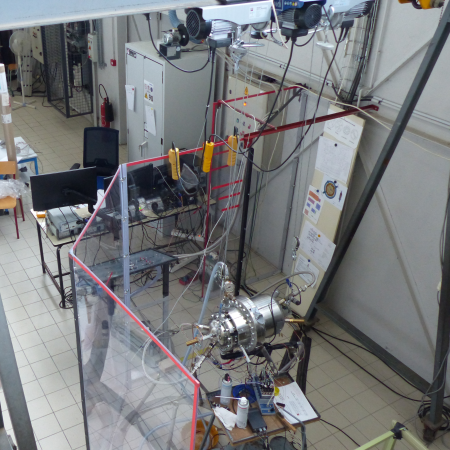
\includegraphics{../fig/fig_BancEssaisComplet/BancEssaisComplet.png}};
	\begin{scope}[x={(image.south east)},y={(image.north west)}]
%		\draw[help lines, xstep=.1, ystep=.1] (0,0) grid (1,1);
		
		\draw[ultra thick, rounded corners, red] (.4,.9) rectangle (.85,1) node[below left, fill=white, fill opacity=.5, text opacity=1]{(a)};% palan
		\draw[ultra thick, rounded corners, red] (.28,.65) -- (.48,.69) -- (.48,.89) node[below left, fill=white, fill opacity=.5, text opacity=1]{(b)} -- (.28,.89) -- cycle;% armoire gaz
		\draw[ultra thick, rounded corners, red] (.65,.61) rectangle (.49,.85) node[below right, fill=white, fill opacity=.5, text opacity=1]{(c)};% armoire electrique
		\draw[ultra thick, rounded corners, red] (.28,.64) -- (.48,.68) |- (.06,.46) |- node[midway, below right, fill=white, fill opacity=.5, text opacity=1]{(d)} (.28,.64) -- cycle;% ordi
		\draw[ultra thick, rounded corners, red] (.4,.45) node[below left, fill=white, fill opacity=.5, text opacity=1]{(e)} rectangle (.15,.35); % tableau gaz
		\draw[ultra thick, rounded corners, red] (.7,.4) -| node[midway, below right, fill=white, fill opacity=.5, text opacity=1]{(f)} (.41,.17) -- (.52,.17) -- (.7,.27) -- cycle;% Tacot
		\draw[ultra thick, rounded corners, red] (.54,.17) -- (.54,.04) node[above right, fill=white, fill opacity=.5, text opacity=1]{(g)} -| (.63,.22) -- cycle;% Baie NI
		
		\draw[very thick, ->, blue] (.8,.1) node(Orig){} node[anchor=east, text=black]{$O$} -- ++(0,.1) node[anchor=south]{$\mathbf e_{z,0}$}; 
		\draw[very thick, ->, red] (Orig.center) -- ++(22.5:.1)node[anchor=south]{$\mathbf e_{x,0}$};
		\draw[very thick, ->, green] (Orig.center) -- ++(-45:.1)node[anchor=south west]{$\mathbf e_{y,0}$};
	\end{scope}
\end{tikzpicture}